% !TeX root = RJwrapper.tex
\title{Round Turn Trade Monte Carlo Simulation in R}
\author{by Jasen Mackie, Author Two}

\maketitle

\abstract{%
With txnsim() the analyst is able to construct a random strategy that
preserves as many of the stylized facts (or style) of the observed
strategy as possible, while demonstrating no skill. The round turn
trades of the random replicate strategies, while outwardly resembling
the original strategy in summary time series statistics, are the result
of random combinations of observed features taking place at random times
in the tested time period. This effectively creates simulated traders
with the same style but without skill. For this reason txnsim() is most
appropriate for discerning skill vs.~luck or overfitting.
}

% Any extra LaTeX you need in the preamble

\hypertarget{introduction}{%
\subsection{Introduction}\label{introduction}}

Introductory section which may include references in parentheses
\citep{R}, or cite a reference such as \citet{R} in the text.

Performance simulations via Monte Carlo and other methods are widely
used in Finance.

\citet{@burns2004} covers the use of random portfolios for performance
measurement and in a subsequent paper in \citet{@burns2006} for
evaluating trading strategies which he terms a related but distinct
task. He goes on to mention in his evaluating strategies paper that
statistical tests for a signal's predictiveness was generally possible
even in the presence of potential data snooping bias. Things have likely
changed in the 14 years since in that data snooping has become more
prevalent, with more data, significantly advanced computing power and
the ability to fit an open source model to almost any dataset. Tomasini
\& Jaeckle in their Trading Systems book \citep{@tomasini2009} refer to
the analysis of trading systems using Monte Carlo analysis of trade PNL.
In particular they mention the benefit of a confidence interval
estimation for max drawdowns. In the Probability of Backtest Overfitting
paper by de Prado et al in 2015 \citep{@bailey2014}, they present a
method for assessing data snooping as it relates to backtests, which are
used by investment firms and portfolio managers to allocate capital.
Harvey et al, in their series of papers including Backtesting
\citep{@harvey2015} and the Cross-Section of Expected Returns
\citep{@harvey2013} discuss their general dismay at the reported
significance of papers attempting to explain the cross-section of
expected returns. They propose a method for deflating the Sharpe Ratio
when taking into account the data snooping bias otherwise referred to as
Multiple Hypothesis testing. Comapared with more well-known simulation
methods, such as simulating portfolio P\&L, Round Turn Trade Simulation
has the following benefits: 1. Increased transparency, since you can
view the simulation detail down to the exact transaction, thereby
comparing the original strategy being simulated to random entries and
exits with the same overall dynamic 2. More realistic since you sample
from trade durations and quantities actually observed inside the
strategy, thereby creating a distribution around the trading dynamics,
not just the daily P\&L What all this means, of course, is you are
effectively creating simulated traders with the same style but zero
skill.

\hypertarget{stylized-facts}{%
\subsection{Stylized facts}\label{stylized-facts}}

If you consider the stylized facts of a series of transactions that are
the output of a discretionary or systematic trading strategy, it should
be clear that there is a lot of information available to work with. The
stylized facts txnsim() uses for simulating round turns include;

\begin{itemize}
\tightlist
\item
  percent time in market (and percent time flat)
\item
  ratio of long to short position taking (in duration terms)
\item
  number of levels or layered trades observed, limited by max position
\end{itemize}

Using these stylized facts, txnsim() samples either with or without
replacement between flat periods, short periods and long periods and
then layers onto these periods the sampled quantities from the original
strategy with their respective durations.

\hypertarget{round-turn-trades-tradedef}{%
\subsection{Round Turn Trades \&
tradeDef}\label{round-turn-trades-tradedef}}

In order to sample round turn trades, the analyst first needs to define
what a round turn trade is for their purposes. In txnsim() there is a
parameter named \emph{tradeDef} which can take one of 3 arguments, 1.
``flat.to.flat'', 2. ``flat.to.reduced'', 3. ``increased.to.reduced''.
The argument is subsequently passed to the blotter::perTradeStats()
function from which we extract the original strategy's stylized facts.
The simplest definition of a round turn trade would be flat.to.flat and
would include all transactions between when a position is opened and
when it is closed. This method is most suitable for a strategy that only
puts on a single level per round turn. This definition would not be
suitable for a strategy that is rarely flat and it would be safe to
assume that most quantitative strategies in production would be using a
variation of position sizing and/or risk management. In the case of
flat.to.reduced a trade's initial entry is always paired with a
transaction which takes the position closer to zero, regardless of any
transactions which may have increased the position along the way.

For increased.to.reduced, every transaction that moves a position closer
to zero will close the round turn. This round turn exit transaction will
be paired with the one or more transactions which take the position
further from zero, thereby locating the initiating transaction/s. This
method is otherwise known as Average Cost First-in First-Out (ACFIFO).

To illustrate the output using either method, we will use a bbands demo
strategy which was slightly amended from the bbands strategy in the demo
folder of the \emph{blotter} package.

If we consider the first 9 transactions in the strategy, from 2007-02-16
to 2007-04-18, we see an example of each round turn trade definition. We
elaborate on this next.

\begin{Schunk}
\begin{Soutput}
#>            Txn.Qty Txn.Price
#> 1950-01-01       0   0.00000
#> 2007-02-16      50  12.11857
#> 2007-02-21      50  12.74286
#> 2007-02-22    -100  12.78714
#> 2007-02-28      50  12.08714
#> 2007-03-02      50  12.20143
#> 2007-03-22    -100  13.42286
#> 2007-03-27    -100  13.63714
#> 2007-04-12      50  13.17000
#> 2007-04-18      50  12.91429
\end{Soutput}
\end{Schunk}

\hypertarget{flat.to.flat}{%
\subsubsection{flat.to.flat}\label{flat.to.flat}}

The first round turn trade using the flat.to.flat definition is composed
of an opening transaction on 2007-02-16 for 50 shares, and a closing
transaction on 2007-02-22 for 100 shares. The layering transaction on
2007-02-21 merely added to the existing position of 50 shares. We store
the \emph{Duration} in seconds to account for higher frequency intraday
strategies. When converted to `days' we see the duration of the first
flat.to.flat period is 6 days.

\begin{Schunk}
\begin{Sinput}
pt_flat.to.flat <- perTradeStats('bbands', 'AAPL', tradeDef = 'flat.to.flat')
head(pt_flat.to.flat[c(1:2,19)],3)
\end{Sinput}
\begin{Soutput}
#>        Start        End     duration
#> 1 2007-02-16 2007-02-22  518400 secs
#> 2 2007-02-28 2007-03-22 1900800 secs
#> 3 2007-03-27 2007-04-18 1900800 secs
\end{Soutput}
\begin{Sinput}
paste0(as.numeric(pt_flat.to.flat$duration[1:3]/86400), " days")
\end{Sinput}
\begin{Soutput}
#> [1] "6 days"  "22 days" "22 days"
\end{Soutput}
\end{Schunk}

\hypertarget{flat.to.reduced}{%
\subsubsection{flat.to.reduced}\label{flat.to.reduced}}

The first round turn trade with a different end date to flat.to.flat is
the trade initiated on 2007-03-27. The intitiating short position for
100 shares is partially unwound for 50 shares on 2007-04-12, which is
the end date for the 3rd round turn trade defined with tradeDef
flat.to.reduced.

\begin{Schunk}
\begin{Sinput}
pt_flat.to.reduced <- perTradeStats('bbands', 'AAPL', tradeDef = 'flat.to.reduced')
head(pt_flat.to.reduced[c(1:2,19)],4)
\end{Sinput}
\begin{Soutput}
#>        Start        End     duration
#> 1 2007-02-16 2007-02-22  518400 secs
#> 2 2007-02-28 2007-03-22 1900800 secs
#> 3 2007-03-27 2007-04-12 1382400 secs
#> 4 2007-03-27 2007-04-18 1900800 secs
\end{Soutput}
\begin{Sinput}
paste0(as.numeric(pt_flat.to.reduced$duration[1:4]/86400), " days")
\end{Sinput}
\begin{Soutput}
#> [1] "6 days"  "22 days" "16 days" "22 days"
\end{Soutput}
\end{Schunk}

\hypertarget{increased.to.reduced}{%
\subsubsection{increased.to.reduced}\label{increased.to.reduced}}

For round turn trade definitions based on increased.to.reduced, any
transaction taking a position closer to zero is paired with one or more
transactions increasing a position. We see 6 round turn trade
observations based on this trade definition during the period 2007-02-16
to 2007-04-18.

\begin{Schunk}
\begin{Sinput}
pt_increased.to.reduced <- perTradeStats('bbands', 'AAPL', tradeDef = 'increased.to.reduced')
head(pt_increased.to.reduced[c(1:2,19)],6)
\end{Sinput}
\begin{Soutput}
#>        Start        End     duration
#> 1 2007-02-16 2007-02-22  518400 secs
#> 2 2007-02-21 2007-02-22   86400 secs
#> 3 2007-02-28 2007-03-22 1900800 secs
#> 4 2007-03-02 2007-03-22 1728000 secs
#> 5 2007-03-27 2007-04-12 1382400 secs
#> 6 2007-03-27 2007-04-18 1900800 secs
\end{Soutput}
\begin{Sinput}
paste0(as.numeric(pt_increased.to.reduced$duration[1:6]/86400), " days")
\end{Sinput}
\begin{Soutput}
#> [1] "6 days"  "1 days"  "22 days" "20 days" "16 days" "22 days"
\end{Soutput}
\end{Schunk}

The most likely trade definitions relevant to strategies observed in
production today are flat.to.flat and increased.to.reduced. For
illustrating the sampling process in txnsim() using flat.to.flat we will
use a slightly amended version of the `longtrend' demo in blotter. It
enters a position only once until an exit signal is triggered and the
entire position is unwound.

Looking at the Position fill window it should be clear the appropriate
trade definition for this strategy is flat.to.flat.

\begin{Schunk}


\begin{center}\includegraphics{RoundTurnTradeMonteCarloSimulation_files/figure-latex/longtrend chart-1} \end{center}

\end{Schunk}

We will use the `bbands' strategy above to illustrate the sampling
process for increased.to.reduced. The same sampling methodology is used
for trade definition flat.to.reduced.

A quick look at the output shows the extent of the layering in this demo
strategy:

\begin{Schunk}
\begin{Sinput}
chart.Posn(Portfolio='bbands',Symbol="AAPL",TA="add_BBands(on=1,sd=SD,n=N)")
\end{Sinput}


\begin{center}\includegraphics{RoundTurnTradeMonteCarloSimulation_files/figure-latex/chart.Posn bbands txnsim demo-1} \end{center}

\end{Schunk}

The below diagram depicts the main functional flow inside txnsim. The
first internal function, \texttt{txnstruct} is used to build a dataframe
of start times, round turn trade durations and quantities. We assign
this to a list named \texttt{backtest.trades} with one element per
symbol in the original portfolio object. We output the backtest.trades
slot in the result of a call to txnsim().

\begin{Schunk}
\begin{Sinput}
lt.wr$backtest.trades
\end{Sinput}
\begin{Soutput}
#> $GSPC
#>         start       duration quantity
#> 1  1998-10-30  28944000 secs       91
#> 2  1999-10-29  29030400 secs       85
#> 3  2002-03-28   2851200 secs      107
#> 4  2003-04-30  39484800 secs      125
#> 5  2004-10-29  97372800 secs      122
#> 6  2009-06-30  28684800 secs      197
#> 7  2010-07-30   2764800 secs      195
#> 8  2010-09-30  28944000 secs      179
#> 9  2012-01-31 113011200 secs      166
#> 10 2015-10-30   5356800 secs      157
#> 11 2016-03-31  55123200 secs      156
#> 12 1999-09-30   2505600 secs        0
#> 13 2000-09-29  47088000 secs        0
#> 14 2002-04-30  31536000 secs        0
#> 15 2004-07-30   7862400 secs        0
#> 16 2007-11-30  49939200 secs        0
#> 17 2010-05-28   5443200 secs        0
#> 18 2010-08-31   2592000 secs        0
#> 19 2011-08-31  13219200 secs        0
#> 20 2015-08-31   5184000 secs        0
#> 21 2015-12-31   7862400 secs        0
\end{Soutput}
\end{Schunk}

Depending on the tradeDef and the bool value for replacement, the
function can take one of 3 routes into a sampling procedure.

\begin{Schunk}
\begin{figure}

{\centering 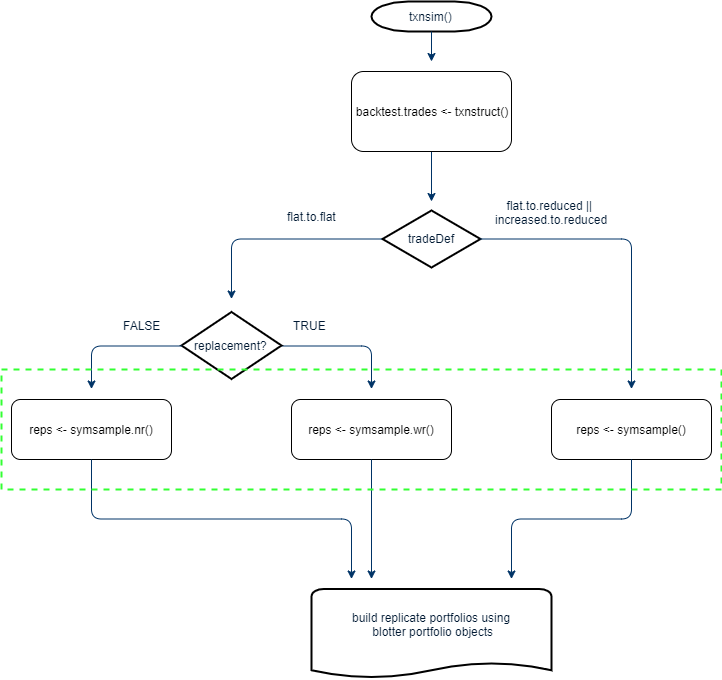
\includegraphics{/home/jmackie/blotter/sandbox/txnsim_flow_diagram} 

}

\caption[Fig.1]{Fig.1. txnsim() - functional flow}\label{fig:txnsim flow diagram diagram}
\end{figure}
\end{Schunk}

\hypertarget{sampling-process}{%
\subsection{Sampling Process}\label{sampling-process}}

The sampling inside txnsim() can happen in 3 mutually exclusive
functions (bordered by the green dotted line), namely:

\begin{enumerate}
\def\labelenumi{\arabic{enumi}.}
\tightlist
\item
  symsample.nr() for tradeDef=``flat.to.flat'' with replacement=FALSE.
\item
  symsample.wr() for tradeDef=``flat.to.flat'' with replacement=TRUE.
\item
  symsample() for tradeDef=``flat.to.reduced'' \textbar{}
  ``increased.to.reduced''. Due to the nature of the tradeDef and the
  fact that strategy total duration will exceed strategy calendar
  duration, sampling only makes sense with replacement=TRUE. Hence there
  is one sampling function for either of these tradeDef's.
\end{enumerate}

\hypertarget{symsample.nr}{%
\subsubsection{symsample.nr}\label{symsample.nr}}

The simplest path to follow inside \texttt{txnsim()} for replicating
strategies is using tradeDef=``flat.to.flat'' without replacement. The
first step inside symsample.nr() is to sample the rows in the
backtest.trades object, without replacement, and then to index those
rows when subsetting from backtest.trades to build our replicate
strategy dataframes of start times, durations and quantities. Since the
sampling happens without replacement the replicate strategies will
exhibit exactly identical durations.

\begin{Schunk}
\begin{figure}

{\centering 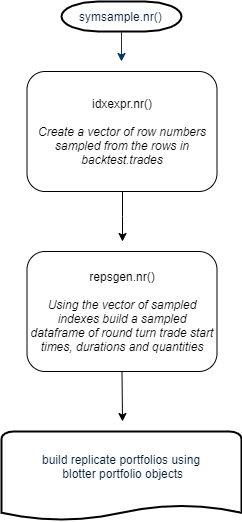
\includegraphics{/home/jmackie/blotter/sandbox/symsample.nr_flow_diagram} 

}

\caption[Fig.2]{Fig.2. symsample.nr() - functional flow}\label{fig:symsample.nr flow diagram diagram}
\end{figure}
\end{Schunk}

\hypertarget{symsample.wr}{%
\subsubsection{symsample.wr}\label{symsample.wr}}

When sampling round turn trades defined as ``flat.to.flat'' but
\emph{with replacement} we have to add a constraint to the sampling of
the originally observed strategy. We apply a ``fudge factor'' of 110\%
to the number of round turns observed in the original strategy (nsamples
= `n' * 1.1), sample `nsamples' times and compare the resulting sum of
durations with the target total duration observed in the original
strategy. If the sum of durations sampled is less than our target
duration, we proceed to sample again, `nsamples' times and compare with
the target duration. We do this in a while loop. Once the sum of sampled
durations exceeds that of our original strategy, we find the row whose
duration takes us over the target duration (since there may be more than
one row), we truncate excess rows and reduce the duration of the row
which takes us over our target duration by the amount required to equal
our target duration. This resulting dataframe becomes our replicate
sampled dataframe of start times, durations and quantities.

\begin{Schunk}
\begin{figure}

{\centering 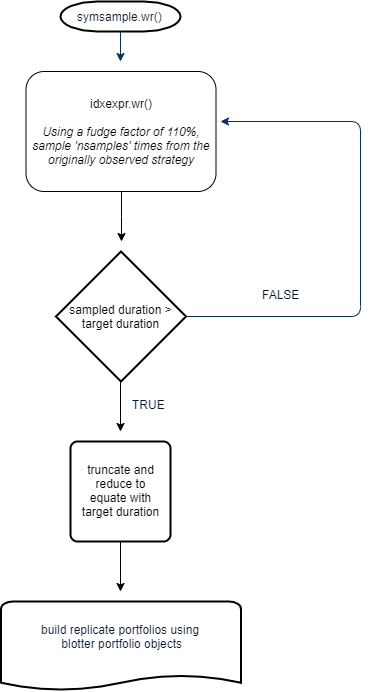
\includegraphics{/home/jmackie/blotter/sandbox/symsample.wr_flow_diagram} 

}

\caption[Fig.3]{Fig.3. symsample.wr() - functional flow}\label{fig:symsample.wr flow diagram diagram}
\end{figure}
\end{Schunk}

\hypertarget{symsample}{%
\subsubsection{symsample}\label{symsample}}

In the event a strategy uses the round turn trade definition of
``increased.to.reduced'' or ``flat.to.reduced'' the function needs to
sample with a few more constraints. Firstly, we need to ensure we do not
over or undersample durations such that the total duration of the
replicate strategy is widely different from the original strategy. The
expectation is that replicates will approach, if not marginally exceed,
the duration of the original strategy. Secondly, when sampling the
quantities to level into an existing position, we need to ensure the
maximum long or short position observed in the strategy is not breached.
We do not know whether or not a strategy employs a max position
constraint, nor any other strategy details. For this reason we measure
the stylized facts exhibited by the strategy and sample within those
constraints.

The sampling is handled by an internal `tradesample()' function. The
first step in this function is to build the first layer of the strategy
with initial entries for long periods, short periods and flat periods.
We use an internal `subsample()' function to perform this task,
shuffling the output such that long, short and flat periods are
intermingled. We store this in a temporary dataframe of start times,
durations and quantities. Positive quantities imply long positions,
negative quantities imply short positions, zero quantities imply flat
periods.

Once we have a first layer we know we have exhausted our flat periods.

For layering onto the first layer we determine firstly whether the total
strategy duration exceeds that of the calendar duration. We store this
value in a variable called num\_overlaps, and check if it is grearter
than 1. If FALSE, there is nothing to layer, and we proceed to building
a replicate portfolio with the output in `tdf' which includes the
sampled start times, durations and quantities. If TRUE, then we proceed
to layering. To start, we establish whether there are any left over long
and/or short round turn trades, that were not included in the sampled
output used for constructing the first layer.

Where there are long round turn trades left over, we prepare a temporary
dataframe using a copy of the first layer. We add a few descriptive
fields to this dataframe, which will help us determine whether or not we
have added a long layer which would overlap into a flat, short or
sequential long periods. We will also update this dataframe as we layer
to determine if the new layered trade, at any point, will take us over
the max position constraint. Since the new layer could overlap multiple
sequential long periods from the first layer, we need to monitor these
positions separately. We repeat this process for short round turn
trades. Below are several examples by way of illustration explaining the
process.

\hypertarget{truncate}{%
\paragraph{Truncate}\label{truncate}}

The simplest scenario for layering is a new layer which overlaps into a
flat or short period. In this case the duration overlapping the end of
the previous layer is truncated.

\begin{Schunk}
\begin{figure}

{\centering 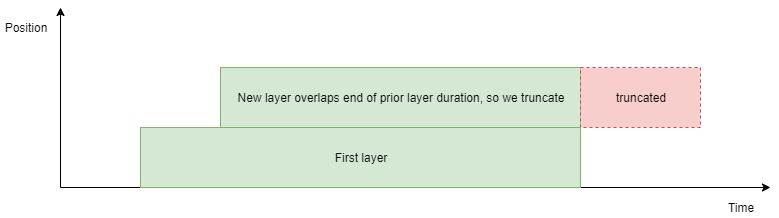
\includegraphics{/home/jmackie/blotter/sandbox/SimpleNewLayer_Truncated} 

}

\caption[Fig.4]{Fig.4. truncate new layer}\label{fig:SimpleNewLayer_Truncated diagram}
\end{figure}
\end{Schunk}

\hypertarget{split}{%
\paragraph{Split}\label{split}}

In scenarios where the new layered trade duration ends before the end of
the prior layer trade duration, we split the prior layer into 2 parts.
The first part will include the newly layered trade and end with the
duration end from the new layer. The first part will include the
quantity from the new layer which will add to the cumulative position of
the replicate strategy and be monitored separately with respect to max
position constraints. The second part will include the portion of the
prior layer which does not include the new layer. Since it is possible
that a new layer may be strapped onto this portion, we need to separate
it in order to monitor the cumulative position with respect to the max
position constraint.

\begin{Schunk}
\begin{figure}

{\centering 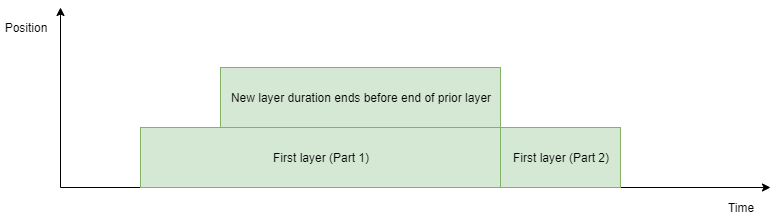
\includegraphics{/home/jmackie/blotter/sandbox/SimpleNewLayer_Split} 

}

\caption[Fig.5]{Fig.5. split prior layer}\label{fig:SimpleNewLayer_Split diagram}
\end{figure}
\end{Schunk}

The above scenarios for truncating a new layer duration or splitting a
prior layer round turn trade assume the prior layer is a single round
turn trade.

\hypertarget{new-layer-overlaps-multiple-prior-layer-segments}{%
\paragraph{New layer overlaps multiple prior layer
segments}\label{new-layer-overlaps-multiple-prior-layer-segments}}

In scenarios where the proposed new layer overlaps more than one
continuous prior period (otherwise referred to as segments) of the same
side, we need to monitor the proposed cumulative position of each
segment individually with respect to max position constraints. The last
prior-layer segment will either be split or the new layer duration
truncated as above.

Figures 6 and 7 below illustrate the scenarios in which a proposed
single new layer (represented with the blue fill) overlaps multiple
individual prior layer segments, each potentially with different
quantities. Before each portion of the new layer can be added, we check
to see it will not breach the original strategy max position observed.
Where a new layer added to a prior segment would breach the observed max
position, the duration is truncated at the start of the segment of the
new layer which would breach the max position constraint.

The example in figure 6 assumes a new layer which overlaps into a flat
period, where the new layer duration is truncated accordingly.

\begin{Schunk}
\begin{figure}

{\centering 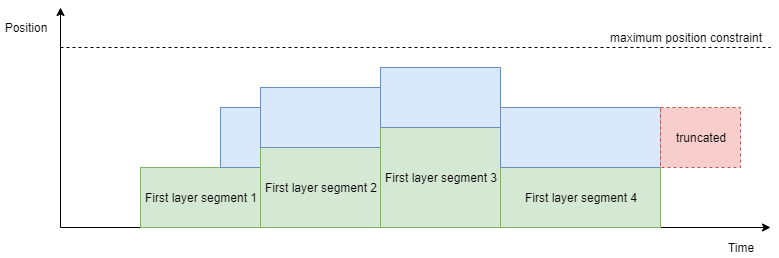
\includegraphics{/home/jmackie/blotter/sandbox/MultiplePriorLayerNewLayer_Truncate} 

}

\caption[Fig.6]{Fig.6. multiple prior layer w/ truncate}\label{fig:MultiplePriorLayerNewLayer_Truncate diagram}
\end{figure}
\end{Schunk}

Figure 7 illustrates the scenario in which a proposed single new layer
(also represented with a blue fill) overlaps multiple individual prior
layer segments but ends before the duration end of the last segment. In
this case, as above in figure 5, we split the last prior-layer,
recording the cumulative position of each segment individually for
future potential new layers with respect to max position constraints.

\begin{Schunk}
\begin{figure}

{\centering 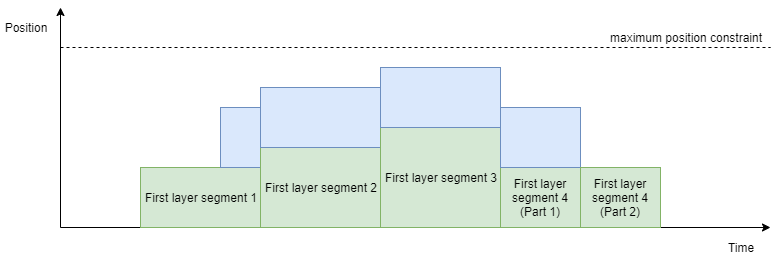
\includegraphics{/home/jmackie/blotter/sandbox/MultiplePriorLayerNewLayer_Split} 

}

\caption[Fig.7]{Fig.7. multiple prior layer w/ split}\label{fig:MultiplePriorLayerNewLayer_Split diagram}
\end{figure}
\end{Schunk}

\hypertarget{sampling-start-times-and-periods-between-start-times}{%
\paragraph{Sampling start times and periods between start
times}\label{sampling-start-times-and-periods-between-start-times}}

In addition to sampling from the observed round turn trade durations and
quantities, we sample from a list of start times, updated with each new
layer start time in our temporary dataframe. In determining how far from
the prior layer start time to start our new layer, we sample from the
range of durations observed between layered trades (recorded separately
for long and short round turn trades) in the original strategy.

Below is a depiction of the logical flow in symsample(). The layering
explained above is depicted in a separate flow diagram in Fig. 9.
{[}TODO: determine whether a flowchart is necessary for the layering
separately\ldots{}{]}

\begin{Schunk}
\begin{figure}

{\centering 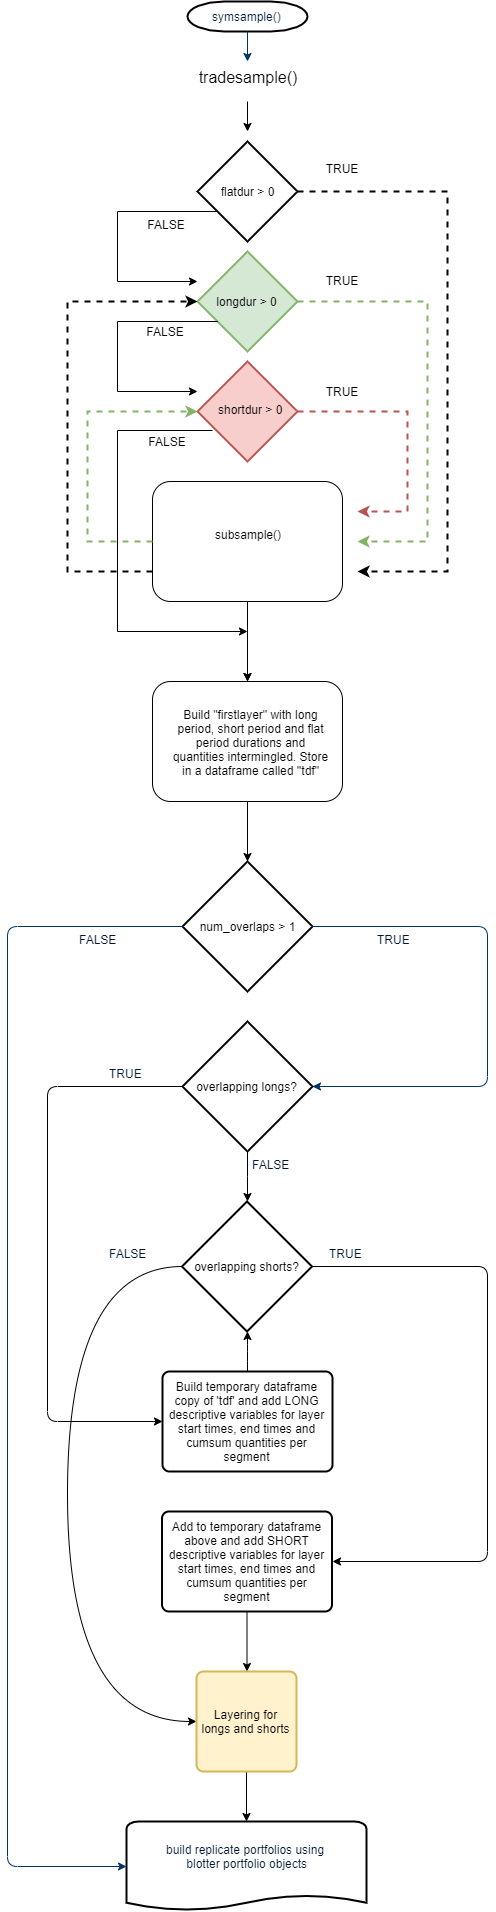
\includegraphics{/home/jmackie/blotter/sandbox/symsample_flow_diagram} 

}

\caption[Fig.8]{Fig.8. symsample() - functional flow}\label{fig:symsample flow diagram diagram}
\end{figure}
\end{Schunk}

TODO: put flowchart here if deemed necessary

\hypertarget{generating-transactions}{%
\subsection{Generating Transactions}\label{generating-transactions}}

Regardless of the round turn trade definition, once the sampling
procedure completes we will have tuples of \emph{start} time,
\emph{duration} and \emph{quantity} for each random replicate of the
original strategy, per symbol, stored in a \emph{reps} object. The index
of each replicate will fit within the original market data index and is
directly observable in the output from a call to txnsim(). Using the
data inside the ``reps'' object we create a series of opening
transactions using the start timestamps and quantities, and create exit
transactions with timestamps equivalent to the start timestamp plus
duration. We assign the relevant price to each proposed transaction with
reference to the market data object in blotter, where open transaction
prices are based on the start timestamp indexes and closing transactions
are based on start timestamp + duration indexes. We convert this series
of opening transactions and closing transactions to an \emph{xts}
object, which is ordered based on time index, and will be used directly
in the \emph{addTxns} function in blotter to generate the entry and exit
transactions.

The transactions are generated in portfolios initialized with names of
the format: ``txnsim'' + rpcstr + original portfolio + replicate number,
where \texttt{rpcstr} is either ``wr'' or ``nr'' indicating whether the
sampling was performed with or without replacement. An example of the
first replicate output from a call to txnsim() on the \texttt{bbands}
strategy without replacement would be ``txnsim.wr.bbands.1''.

\hypertarget{output}{%
\subsubsection{Output}\label{output}}

\emph{To illustrate the output from txnsim() I will use the same 2
sample strategy backtests from above, the first being a slight variation
of the
\href{https://github.com/braverock/blotter/blob/master/demo/longtrend.R}{`longtrend'}
demo in the blotter package and the second a variation of the
\href{https://github.com/braverock/quantstrat/blob/master/demo/bbands.R}{`bbands'}
demo from the quantstrat package. In both instances I use a fixed end
date (2017-12-31) for the purposes of replication. In addition, for
bbands I vary the exit quantity of shares in order to generate a
backtest with layers thereby illustrating how txnsim() honors these
layers when building random replicates.}

As with mcsim(), txnsim() uses S3 methods for plotting the replicate
equity curves and summary statistic histograms. Before delving into
those and the other methods and slots in txnsim(), a quick overview of
the `longtrend' strategy itself may be appropriate.

Based on the strategy covered in Faber's paper
\href{https://papers.ssrn.com/sol3/papers.cfm?abstract_id=962461}{A
Quantitative Approach to Tactical Asset Allocation} Faber looks to test
a trend following system similar to that covered by Jeremy Siegel in
``Stocks for the Long Run''. Siegel tests a simple 200-day moving
average strategy on the DJIA since 1885 and concludes that using the
long-term moving average strategy an investor is able to outperform a
buy-and-hold strategy on a risk-adjusted basis after transaction costs.
Faber tests a similar strategy but using monthly data and the 10-month
moving average of the S\&P500 since 1901, and since 1973 for the
``Global Tactical Asset Allocation (GTAA)'' portfolio. Their use of
monthly data is due to a restriction on the availability of data for
their extension of the strategy to multi-asset class portfolios. The
lower periodicity however has the added benefit of reducing transaction
costs. Faber's results show the timing model outperforming a
buy-and-hold strategy on the S\&P500 as well as when applied to an
equally weighted portfolio of 5 different asset classes on a
risk-adjusted and absolute returns basis.

Taking a look at the `longtrend' equity curve, its clear the strategy
benefitted from being out the market during the protracted bear markets
following the tech and housing bubbles. For this reason trend following
systems add the most value when applied over entire busines cycles.

\begin{Schunk}


\begin{center}\includegraphics{RoundTurnTradeMonteCarloSimulation_files/figure-latex/longtrend equity_curve-1} \end{center}

\end{Schunk}

For a more holistic view of the strategy performance and time in the
market we call \emph{chart.Posn()}. The flat periods during the
protracted bear markets should be more evident looking at the position
fill window.

\begin{Schunk}


\begin{center}\includegraphics{RoundTurnTradeMonteCarloSimulation_files/figure-latex/longtrend chart_again-1} \end{center}

\end{Schunk}

Using txnsim() we are able to measure the performance of any number of
randomized versions of this `longtrend' strategy. Below is a visual
comparison of the orignal strategy's equity curve and 1k random
replicate equity curves with and without replacement.

\begin{Schunk}


\begin{center}\includegraphics{RoundTurnTradeMonteCarloSimulation_files/figure-latex/longtrend_txnsim-1} \end{center}



\begin{center}\includegraphics{RoundTurnTradeMonteCarloSimulation_files/figure-latex/longtrend_txnsim-2} \end{center}

\begin{Soutput}
#> Time difference of 0.5874317 secs
\end{Soutput}
\end{Schunk}

Interestingly, the `longtrend' strategy appears difficult to beat at
random when constrained by the same characteristics as the original
strategy. There are some ``lucky'' traders which manage to outperform
`longtrend' for a period until close to the end of the strategy when in
early 2016 and until the end of the backtest period `longtrend' is long
and benefits from the 2016/2017 bull market. In terms of totalPL
`longtrend' ranks 12th to eleven
\href{http://www.followingthetrend.com/2016/04/you-cant-beat-all-the-chimps/}{very
lucky chimps}. Of course many of the random traders would have been
disadvantaged by taking positions during the deep drawdowns experienced
following the tech and housing bubbles or being flat during the
2016-2017 bull market, but their time in the market would resemble the
same characteristics as `longtrend' itself. We can take a look at the
position chart of any one of the replicates to get a sense of how the
respective random trader did. It should also illustrate how txnsim()
honors the characteristics of the original strategy in terms of time in
and out the market and quantities traded. Of course there is no layering
in `longtrend' nor are there any short trades, so we expect to see 1
level of long positions for a similar total duration as the original
strategy.

\begin{Schunk}
\begin{Sinput}
chart.Posn("txnsim.wr.longtrend.1", Symbol = "GSPC")
\end{Sinput}


\begin{center}\includegraphics{RoundTurnTradeMonteCarloSimulation_files/figure-latex/longtrend_txnsim 1st replicate-1} \end{center}

\end{Schunk}

From the analysis thus far we are able to deduce that our `longtrend'
strategy outperformed 983 random traders (out of 1,000) on a totalPL
basis, following the same style. It would be difficult to conclude that
the performance from `longtrend' is the result of chance, since the
strategy of long-term trend following has been used for decades for a
reason. The benefits from being invested in risk-free assets during
economic downturns cannot be understated. Indeed, the strategy's
outpeformance increases over time as evidenced in the equity curve plot
\emph{(plot(lt.wr))} as many different market regimes are experienced.
Could we have overfit the backtest? Referring to Faber's paper, he finds
stability in his results for the GTAA portfolio when analyzing the range
of monthly moving averages from 3m-12m. The analyst could easily perform
a similar analysis using the
\href{https://github.com/braverock/quantstrat/blob/master/R/paramsets.R}{\emph{apply.paramset}}
function in quantstrat. Ignoring the many other potential objectives for
assessing a strategy's feasibility for promotion to a production
environment, `longtrend' seems to pass initial scrutiny.

\hypertarget{ranks-and-p-values}{%
\subsubsection{Ranks and p-values}\label{ranks-and-p-values}}

One of the slots in the return object from txnsim() are the ranks of
each replicate and the original strategy in terms of the summary
statistics. The original strategy will be the first row in the
dataframe. These ranks are used to determine the p-values of the
statistics, in which p-values are calculated with reference to
\href{https://www.ncbi.nlm.nih.gov/pmc/articles/PMC379178/}{North et.
al. (2002)} who use Davison \& Hinkley (1997) as their source.

\begin{Schunk}
\begin{Sinput}
head(lt.wr$ranks, 10)
\end{Sinput}
\begin{Soutput}
#>                       mean median stddev maxDD sharpe totalPL
#> longtrend                1      7      8     1      1       1
#> txnsim.wr.longtrend.1    5      7      9     2      2       5
#> txnsim.wr.longtrend.2   10      7     11     4      8      10
#> txnsim.wr.longtrend.3    7      7      7     6      7       7
#> txnsim.wr.longtrend.4    9      7     10     5      9       9
#> txnsim.wr.longtrend.5    2      2      2     8      4       2
#> txnsim.wr.longtrend.6   11      7      6     7     11      11
#> txnsim.wr.longtrend.7    4      7      1    10      5       4
#> txnsim.wr.longtrend.8    6      7      3    11      6       6
#> txnsim.wr.longtrend.9    8      7      5     9     10       8
\end{Soutput}
\begin{Sinput}
lt.wr$pvalues
\end{Sinput}
\begin{Soutput}
#>    mean  median  stddev   maxDD  sharpe totalPL 
#>    0.09    0.64    0.73    0.09    0.09    0.09
\end{Soutput}
\end{Schunk}

Since we have the statistic ranks of each replicate in a dataframe, it
is possible to identify which replicates outperformed our original
strategy based on either statistic. The below replicates outperformed
`longtrend' on a totalPL basis.

\begin{Schunk}
\begin{Sinput}
lt.wr$ranks[,6][which(lt.wr$ranks[,6] < 16)][order(lt.wr$ranks[,6][which(lt.wr$ranks[,6] < 16)])]
\end{Sinput}
\begin{Soutput}
#>              longtrend  txnsim.wr.longtrend.5 txnsim.wr.longtrend.10  txnsim.wr.longtrend.7  txnsim.wr.longtrend.1 
#>                      1                      2                      3                      4                      5 
#>  txnsim.wr.longtrend.8  txnsim.wr.longtrend.3  txnsim.wr.longtrend.9  txnsim.wr.longtrend.4  txnsim.wr.longtrend.2 
#>                      6                      7                      8                      9                     10 
#>  txnsim.wr.longtrend.6 
#>                     11
\end{Soutput}
\end{Schunk}

One of the benefits mentioned previously for simulating round turn
trades versus portfolio PL is the transparency. For a closer look at the
winning random replicate we can analyse the trade durations and
quantities using \emph{chart.Posn()}.

\begin{Schunk}
\begin{Sinput}
win_rep <- names(lt.wr$ranks[,6][which(lt.wr$ranks[,6] == 1)])
chart.Posn(win_rep, Symbol = "GSPC")
\end{Sinput}


\begin{center}\includegraphics{RoundTurnTradeMonteCarloSimulation_files/figure-latex/longtrend_txnsim best totalPL replicate-1} \end{center}

\end{Schunk}

\hypertarget{hist.txnsim}{%
\subsubsection{hist.txnsim()}\label{hist.txnsim}}

With the hist.txnsim() method the analyst can generate a histogram from
5 different summary statistics: mean return, median return, max
drawdown, standard deviation and sharpe ratio. The statistics are based
on daily periodicities, and can be normalized or left as the default
cash returns.

Looking at the risk adjusted return we see our `longtrend' demo is close
to the top of the distribution, well ahead of the upper confidence
interval which was left as the default 95\%.

\begin{Schunk}
\begin{Sinput}
hist(lt.wr, methods = "sharpe")
\end{Sinput}


\begin{center}\includegraphics{RoundTurnTradeMonteCarloSimulation_files/figure-latex/longtrend_txnsim hist_sharpe-1} \end{center}

\end{Schunk}

For max drawdown, since we missed the deep drawdowns in 2001-2002 and
2008, we expect to be close to the upper bound of that distribution too.

\begin{Schunk}
\begin{Sinput}
hist(lt.wr, methods = "maxDD")
\end{Sinput}


\begin{center}\includegraphics{RoundTurnTradeMonteCarloSimulation_files/figure-latex/longtrend_txnsim hist_maxDD-1} \end{center}

\end{Schunk}

The `longtrend' strategy may not be the most appropriate for determining
luck versus skill or overfitting with txnsim since random traders would
be locked into their trades for lengthy durations thanks to the monthly
periodicity of the signal process. Nevertheless using txnsim() we are
able to dissect the performance of the strategy over its random
counterparts and in so doing ascertain some level of confidence in the
merits of this particular trend following strategy. Applying the
analysis to a portfolio of asset classes may be an insightful
undertaking.

\hypertarget{another-perspective-using-mcsim}{%
\subsubsection{Another perspective using
mcsim()}\label{another-perspective-using-mcsim}}

For an idea of the possible paths the daily equity curve could have
taken, we also have the option of calling mcsim() without replacement
and comparing the results of a portfolio PL simulation. A look at how
the strategy compares in terms of maximum drawdown may add value to the
analysis.

\begin{Schunk}
\begin{Sinput}
set.seed(333) #for the purposes of replicating my results
lt.mcsim.wr <- mcsim('longtrend', n = 1000)
plot(lt.mcsim.wr)
\end{Sinput}


\begin{center}\includegraphics{RoundTurnTradeMonteCarloSimulation_files/figure-latex/longtrend_mscim-1} \end{center}

\begin{Sinput}
hist(lt.mcsim.wr, methods = "mean", normalize = FALSE)
\end{Sinput}


\begin{center}\includegraphics{RoundTurnTradeMonteCarloSimulation_files/figure-latex/longtrend_mscim-2} \end{center}

\begin{Sinput}
hist(lt.mcsim.wr, methods = "maxDD", normalize = FALSE)
\end{Sinput}


\begin{center}\includegraphics{RoundTurnTradeMonteCarloSimulation_files/figure-latex/longtrend_mscim-3} \end{center}

\begin{Sinput}
print(lt.mcsim.wr, normalize = FALSE)
\end{Sinput}
\begin{Soutput}
#>        Sample Mean Sample Median   Backtest   Lower CI   Upper CI Std. Error
#> mean      1394.923      1391.495   1378.020    704.655   2085.191    352.184
#> median      63.821         0.000      0.000   -375.586    503.229    224.192
#> stddev    5445.826      5441.503   5477.659   4758.775   6132.877    350.543
#> maxDD   -38041.291    -35804.649 -29356.796 -62726.819 -13355.764  12594.888
#> sharpe       0.258         0.256      0.252      0.122      0.393      0.069
\end{Soutput}
\end{Schunk}

Looking at the results of mcsim() on the `longtrend' demo the return and
drawdown characteristics of the original strategy are certainly
reasonable, with both metrics closer to the average of the simulations
compared with txnsim(). Of course maxixmum drawdown is slightly better
than the average which should be expected for a trend following
strategy.

\hypertarget{print.txnsim}{%
\subsubsection{print.txnsim()}\label{print.txnsim}}

Lastly for `longtrend' we look at a summary of the backtest and
replicate summary statistics using the print.txnsim() S3 method. It is a
wrapper for the summary.txnsim() method, so calling print(lt.wr) will be
sufficient for viewing a summary of the results.

\begin{Schunk}
\begin{Sinput}
print(lt.wr)
\end{Sinput}
\begin{Soutput}
#>           backtest Std. Error    Lower CI   Upper CI
#> mean      1378.020    374.085     -32.288   1434.099
#> median       0.000    260.510    -402.663    618.519
#> stddev    5477.659    871.925    4638.277   8056.161
#> maxDD   -29356.796  31930.067 -163520.951 -38357.390
#> sharpe       0.252      0.063      -0.011      0.234
#> totalPL 318322.527  87586.686   -4576.863 338756.639
\end{Soutput}
\end{Schunk}

\hypertarget{layers-and-longshort-strategies-with-bbands}{%
\subsubsection{Layers and Long/Short strategies with
`bbands'}\label{layers-and-longshort-strategies-with-bbands}}

To highlight the ability of txnsim() to capture the stylized facts of
more comprehensive strategies including Long/Short strategies with
leveling we use a variation of the `bbands' strategy. Since we apply an
un-optimised position-sizing adjustment to illustrate leveling, we do
not expect the strategy to outperform the majority of its random
counterparts.

A call to \emph{chart.Posn} highlights the additional traits, namely
entering long \textbf{and} short positions \textbf{with leveling} in and
out, when compared with `longtrend'.

\begin{Schunk}
\begin{Sinput}
chart.Posn(Portfolio='bbands',Symbol="AAPL",
           TA="add_BBands(on=1,sd=SD,n=N)")
\end{Sinput}


\begin{center}\includegraphics{RoundTurnTradeMonteCarloSimulation_files/figure-latex/bbands chart and equity curve-1} \end{center}

\end{Schunk}

\hypertarget{a-thousand-random-traders}{%
\subsubsection{A thousand random
traders}\label{a-thousand-random-traders}}

We run 1000 replicates from a slight variation on the `bbands'
quantstrat demo strategy to generate simulations for 1000 random traders
using \emph{txnsim}.

The \emph{txnsim} function can be fairly CPU and memory intensive. We
have observed 1k replicates taking anywhere from less than 10 minutes on
a large research PC to several hours on less capable hardware {[}TODO:
test on my laptop{]}.

\begin{Schunk}


\begin{center}\includegraphics{RoundTurnTradeMonteCarloSimulation_files/figure-latex/bbands_txnsim plot-1} \end{center}

\begin{Soutput}
#> Time difference of 8.337038 secs
\end{Soutput}
\end{Schunk}

The resulting equity curves confirm our suspicions that we have a lower
probability of outperforming random replicates for this version of
`bbands'.

Taking a closer look at the performance and position taking of the
``winning'' random replicate, we get a sense of how the strategy
attempts to mirror the original in terms of position sizing and duration
of long versus short positions overall. It should also be evident how
the replicate has honored the maximum long and short positions observed
in the original strategy.

\begin{Schunk}
\begin{Sinput}
win_rep <- names(bb.wr$ranks[,6][which(bb.wr$ranks[,6] == 1)])
chart.Posn(win_rep, Symbol = "AAPL") 
\end{Sinput}


\begin{center}\includegraphics{RoundTurnTradeMonteCarloSimulation_files/figure-latex/bbands_txnsim best totalPL replicate-1} \end{center}

\end{Schunk}

Below is another view of the Positionfill segment in the above chart.

\begin{Schunk}


\begin{center}\includegraphics{RoundTurnTradeMonteCarloSimulation_files/figure-latex/bbands_txnsim PositionFill-1} \end{center}

\end{Schunk}

\hypertarget{txnsim---the-process}{%
\subsubsection{txnsim - the process}\label{txnsim---the-process}}

As alluded to in the \emph{Round Turn Trades \& tradeDef} and
\emph{Sampling Process} sections, there are 3 basic variations for
sampling round turn trades in txnsim.

\hypertarget{flat.to.flat-replace-false}{%
\paragraph{1. ``flat.to.flat'' \&\& replace =
FALSE}\label{flat.to.flat-replace-false}}

The simplest case would be sampling round turns defined as
``flat.to.flat'' without replacement. In this case we would simply be
rearranging the vector of durations and quantities. The paths which the
resulting equity curves can take will vary together with the final
result, since we will be marking the simulated trades to market data
timestamps based on randomly sampled durations.

Using the \emph{replicates} slot returned in the output of txnsim, we
can analyze the stylized facts used to build the \emph{transactions}
which are also returned as a slot in the txnsim object. Any timestamp
variation between replicates and transactions will most probably stem
from replicate timestamps falling on weekends or holidays, or due to
missing market data such as in the case of a strategy with a monthly
periodicity and corresponding monthly market data (such as the longtrend
demo). In these cases the transaction will be added at the most recent
timestamp with market data.

Looking at the sum of long period durations from the original strategy
as well as for the first 2 replicates should highlight how txnsim honors
this stylized fact when building out the replicates using
tradeDef=flat.to.flat and replace=FALSE for our `longtrend' example.

\begin{Schunk}
\begin{Soutput}
#> 
#>  4995 long period duration for original strategy 
#>  
#>  4995 long period duration for replicate 1 
#>  
#>  4995 long period duration for replicate 2
\end{Soutput}
\end{Schunk}

\hypertarget{flat.to.flat-replace-true}{%
\paragraph{2. ``flat.to.flat'' \&\& replace =
TRUE}\label{flat.to.flat-replace-true}}

The next simplest case for simulating round turn trades is sampling
``flat.to.flat'' round turns with replacement. Since we will inevitably
be sampling a particular duration multiple times, it is possible to end
with a total duration greater than or less than the original strategy
total duration. To manage this risk we, 1. add a ``fudge factor'' to the
size of our sample and, 2. keep sampling until the sampled total
duration is equal to or exceeds our target total duration (the total
duration from the original strategy).

After sampling the resultant durations we identify which n-th element in
the vector takes us over our target duration, truncate any element
beyond that and trim the duration in the n-th element to get a newly
sampled dataframe of durations and their respective quantities which
matches the total duration of the original strategy.

Since we have sampled with replacement, our replicates will have a range
of long and flat period durations centered around the long and flat
period durations from `longtrend' itself. Before building a histogram to
show these distributions, a quick look at the sum of long period
durations and flat period durations from a few replicates is worthwhile.

\begin{Schunk}
\begin{Soutput}
#> 
#>  4995 long period duration for original strategy 
#>  2005 flat period duration for original strategy 
#>  7000 total duration 
#>  
#>  5277 long period duration for replicate 1 
#>  1723 flat period duration for replicate 1 
#>  7000 total duration 
#>  
#>  6211 long period duration for replicate 5 
#>  789 flat period duration for replicate 5 
#>  7000 total duration 
#>  
#>  6239 long period duration for replicate 10 
#>  761 flat period duration for replicate 10 
#>  7000 total duration
\end{Soutput}
\end{Schunk}

The histogram below confirms the normal distribution around which our
longtrend demo long period duration is centered.

\begin{Schunk}

\includegraphics{RoundTurnTradeMonteCarloSimulation_files/figure-latex/histogram long period durations longtrend_txnsim flat.to.flat with replacement-1} \end{Schunk}

By implication the flat period durations will display an equivalent
distribution around the sum of our longtrend demo flat durations.

\begin{Schunk}

\includegraphics{RoundTurnTradeMonteCarloSimulation_files/figure-latex/histogram flat period durations longtrend_txnsim flat.to.flat with replacement-1} \end{Schunk}

\hypertarget{increased.to.reduced-flat.to.reduced}{%
\paragraph{3. ``increased.to.reduced'' \textbar{}\textbar{}
``flat.to.reduced''}\label{increased.to.reduced-flat.to.reduced}}

For any round turn trade methodology which is not measuring round turns
as flat.to.flat, things get more complicated. Fortunately, the
complication is the same for txnsim regardless of the methodology used
to pair entry and exit trades.

The first major complication with any trade that levels into a position
is that the sum of trade durations will be longer than the market data.
The general pattern of the solution to this complication is that we
sample as usual, to a duration eqivalent to the duration of the first
layer of the strategy. In essence we are sampling assuming round turns
are defined as ``flat.to.flat''. Any sampled durations beyond this first
layer are overlapped onto the first layer. We continue to layer as long
as the replicate strategy duration is below the original, or is unable
to match the original strategy after 1k loops {[}TODO: make this 1k
dynamic to the strategy market data{]}. In this way the total number of
layers and their duration is directly related to the original strategy.

The next complication is max position. Now, a strategy may or may not
utilize position limits. This is irrelevant. We have no idea which
parameters are used within a strategy, only what is observable ex post.
For this reason we store the maximum long and short positions observed
as a stylized fact. To ensure we do not breach these observed max long
and short positions during layering we keep track of the respective
cumsum of each long and short levelled trade.

The procedure for building the first layer in a replicate strategy using
tradeDef=``increased.to.reduced'' is slightly different to the procedure
for building replicates when tradeDef=``flat.to.flat''. For
``flat.to.flat'' round turns, it is perfectly suitable to sample care
free between flat, long and short periods with their respective
quantities. For any trade definition other than flat.to.flat, however,
we need to be cogniscant of flat periods when layering to ensure we do
not layer into an otherwise sampled flat period. For this reason we
match the sum duration of flat periods in the original strategy for
every replicate. To complete the first layer with long and short
periods, we sample these separately and truncate the respectively
sampled long and short duration which takes us over our target duration.
When determining a target long and short total duration to sample to, we
use the ratio of long periods to short periods from the original
strategy to distinguish between the direction of non-flat periods.

At this point it would be worth taking a look at a few \emph{first
layer} replicate flat, long and short durations before looking at their
total distributions. We expect the first layer distributions to be
tightly centered around the original strategy. This is because we
secured the flat periods per the original strategy and used the
long:short ratio stylized fact \emph{(lsratio)} to target sample first
layer long and short durations (the sum of which may not exceed the
calendar duration of the original strategy). The variation for long and
short durations will stem from the fact that we truncate completely the
duration which takes us over our target for long and short duration
sampling.

\begin{Schunk}
\begin{Soutput}
#> 
#>  2398 first layer long period duration for original strategy 
#>  584 first layer flat period duration for original strategy 
#>  987 first layer short period duration for original strategy 
#>  3969 total duration of first layer 
#>  
#>  7055 first layer long period duration for replicate 1 
#>  584 first layer flat period duration for replicate 1 
#>  2456 first layer short period duration for replicate 1 
#>  10095 total duration of first layer 
#>  
#>  7035 first layer long period duration for replicate 2 
#>  584 first layer flat period duration for replicate 2 
#>  2307 first layer short period duration for replicate 2 
#>  9926 total duration of first layer
\end{Soutput}
\end{Schunk}

The replicate flat periods are each 584 days and identical to the
original strategy. Due to truncation, the first layer long and short
periods will vary but to a much lesser extent than with
tradeDef=``flat.to.flat'' with replacement. Of course, when comparing
the total duration of each strategy including their respective layers,
the distribution will fan out somewhat. Let's look at the long and short
period distributions of each replicate for all layers combined.

\begin{Schunk}

\includegraphics{RoundTurnTradeMonteCarloSimulation_files/figure-latex/histogram long period durations bbands_txnsim with replacement-1} \end{Schunk}

\begin{Schunk}

\includegraphics{RoundTurnTradeMonteCarloSimulation_files/figure-latex/histogram short period durations bbands_txnsim with replacement-1} \end{Schunk}

The above histograms highlight how the observed durations from our
bbands demo are quite far removed from the distribution of the random
replicates themselves, which derive directly from the bbands demo. Our
layering procedure inside txnsim may need to capture more granularly the
structure of the layering in the observed strategy. At present we
essentially sample randomly between 2 points to determine the start time
of a layered trade. Future work on txnsim will most likely focus on this
perceived shortcoming, to better capture the style of the original
strategy where tradeDef=``increased.to.reduced''.

\hypertarget{future-work}{%
\subsubsection{Future Work}\label{future-work}}

This research area is full of pitfalls and opportunities. Using the
simulation to try to replicate stylized facts is a series of tradeoffs.
Each stylized fact adds more realism to the simulated random traders,
but also runs the risk of overfitting to the behavior of the original
observed series of trades. For example, as of January 2018, the trade
layering simulations systematically under-represent the amount of time
the simulation takes a larger position, in comparison to the observed
trades. We feel that this particular problem is solvable, but other
simulation difficulties are sure to arise as other stylized facts are
considered for inclusion in later versions.

There are other simulation methodologies still to be implemented,
including Combinatorially Symmetric Cross-Validation (CSCV per Bailey
and Lopez de Prado), various drawdown analysis simulation metrics,
simulations using simulated or resampled market data, application of the
\emph{txnsim} stylized facts to other market data than the original
observed data, and more.

Further, though some methods for doing so are already implemented in
\emph{quantstrat}, there is more work to be done in evaluating whether a
series of observed transactions are likely to be overfit.

In round turn trade simulation, there may be utility in allowing the
analyst to choose which stylized facts to attempt to replicate or use in
the simulation. There may also be value in providing the stylized fact
functions as exposed user functions that could be called on an observed
set of transactions without doing any simulation, just for descriptive
purposes.

\hypertarget{conclusion}{%
\subsubsection{Conclusion}\label{conclusion}}

Round turn trade Monte Carlo simulates random traders who behave in a
similar manner to an observed series of real or backtest transactions.
We feel that round turn trade simulation offers insights significantly
beyond what is available from:

\begin{itemize}
\tightlist
\item
  equity curve Monte Carlo (implemented in \emph{blotter} in
  \emph{mcsim}),
\item
  from simple resampling (e.g.~from \emph{pbo} or \emph{boot}),
\item
  or from the use of simulated input data (which typically fails to
  recover many important stylized facts of real market data).
\end{itemize}

Round turn trade Monte Carlo as implemented in \emph{txnsim} directly
analyzes what types of trades and P\&L were plausible with a similar
trade cadence to the observed series. It acts on the same real market
data as the observed trades, efficiently searching the feasible space of
possible trades given the stylized facts. It is, in our opinion, a
significant contribution for any analyst seeking to evaluate the
question of ``skill vs.~luck'' of the observed trades, or for more
broadly understanding what is theoretically possible with a certain
trading cadence and style.

\hypertarget{references}{%
\subsection{References}\label{references}}

Burns, Patrick. 2004. ``Performance Measurement Via Random Portfolios.''
\url{https://papers.ssrn.com/sol3/papers.cfm?abstract_id=630123}

Burns, Patrick. 2006. ``Random Portfolios for Evaluating Trading
Strategies.''
\url{http://www.burns-stat.com/pages/Working/evalstrat.pdf}

Tomasini, Emilio \& Jaekle, Urban. 2009. ``Trading Systems: A New
Approach to System Development and Portfolio Optimization''

Bailey, David H, Jonathan M Borwein, Marcos López de Prado, and Qiji Jim
Zhu. 2014. ``The Probability of Backtest Overfitting.''
\url{http://papers.ssrn.com/sol3/papers.cfm?abstract_id=2326253}.

Harvey, Campbell R., and Yan Liu. 2015. ``Backtesting.'' SSRN.
\url{http://ssrn.com/abstract=2345489}.

Peterson, Brian G. 2017. ``Developing \& Backtesting Systematic Trading
Strategies.'' \url{http://goo.gl/na4u5d}

\hypertarget{another-section}{%
\subsection{Another section}\label{another-section}}

There will likely be several sections, perhaps including code snippets,
such as:

\begin{Schunk}
\begin{Sinput}
x <- 1:10
x
\end{Sinput}
\begin{Soutput}
#>  [1]  1  2  3  4  5  6  7  8  9 10
\end{Soutput}
\end{Schunk}

\hypertarget{summary}{%
\subsection{Summary}\label{summary}}

This file is only a basic article template. For full details of
\emph{The R Journal} style and information on how to prepare your
article for submission, see the
\href{https://journal.r-project.org/share/author-guide.pdf}{Instructions
for Authors}.

\bibliography{RJreferences}


\address{%
Jasen Mackie\\
Affiliation\\
line 1\\ line 2\\
}
\href{mailto:jasen.mackie@iress.com}{\nolinkurl{jasen.mackie@iress.com}}

\address{%
Author Two\\
Brian G. Peterson\\
line 1\\ line 2\\
}
\href{mailto:author2@work}{\nolinkurl{author2@work}}

